\documentclass[conference]{IEEEtran}
\usepackage[T1]{fontenc}
\usepackage{amsmath,amssymb,graphicx,booktabs,array,tabularx,xspace,cite,url}
\usepackage[hidelinks]{hyperref}
\newcolumntype{Y}{>{\raggedright\arraybackslash}X}
\newcommand{\Ehat}{\widehat E}
\newcommand{\AG}{\textsc{Agreement}}
% Generated by scripts/extract_results.py; do not hand-edit.
\newcommand{\BaselineRuns}{400\xspace}
\newcommand{\SuccessRuns}{366\xspace}
\newcommand{\BudgetRuns}{34\xspace}
\newcommand{\PrimaryModelPercent}{92.80\xspace}
\newcommand{\PrimaryEmpiricalPercent}{91.50\xspace}
\newcommand{\PrimaryCILower}{88.36\xspace}
\newcommand{\PrimaryCIUpper}{93.85\xspace}
\newcommand{\PrimaryDeviationPP}{1.30\xspace}
\newcommand{\TotalUpdates}{13,518\xspace}
\newcommand{\TotalEvaluations}{40,554\xspace}
\newcommand{\TotalMeasurements}{121,662\xspace}
\newcommand{\TotalShots}{124,581,888\xspace}
\newcommand{\ModelStates}{262,144\xspace}
\newcommand{\ModelTransitions}{755,176\xspace}
\newcommand{\GridPoints}{65,536\xspace}
\newcommand{\SuccessPoints}{8\xspace}
\newcommand{\GroundEnergy}{-0.702930394\xspace}
\newcommand{\ShotsPerGroup}{1,024\xspace}
\newcommand{\ShotsPerUpdate}{9,216\xspace}
\newcommand{\MaxShotsRun}{460,800\xspace}
\newcommand{\UpdateBound}{50\xspace}
\newcommand{\GridSize}{16\xspace}
\newcommand{\GapThreshold}{0.02\xspace}
\newcommand{\QuadraturePoints}{24\xspace}
\newcommand{\BootstrapSamples}{5,000\xspace}
\newcommand{\LogicalProperties}{7\xspace}
\newcommand{\DafnyChecks}{24\xspace}
\newcommand{\PModelMean}{33.111\xspace}
\newcommand{\PEmpiricalMean}{32.290\xspace}
\newcommand{\PMeanLow}{31.579\xspace}
\newcommand{\PMeanHigh}{32.995\xspace}
\newcommand{\PMeanRawP}{0.024\xspace}
\newcommand{\PMeanAdjustedP}{0.094\xspace}
\newcommand{\UnconditionalModel}{34.327\xspace}
\newcommand{\UnconditionalEmpirical}{33.795\xspace}
\newcommand{\EnergyError}{5.542\times 10^{-17}\xspace}
\newcommand{\StormDifference}{1.110\times 10^{-16}\xspace}
\newcommand{\QuadratureCorrection}{5.090\times 10^{-8}\xspace}
\newcommand{\DetectablePP}{3.62\xspace}
\newcommand{\LegacyLogicalProperties}{41\xspace}
\newcommand{\PhaseQueries}{18\xspace}
\newcommand{\TimingMeasured}{300\xspace}
\newcommand{\TimingWarmup}{50\xspace}
\newcommand{\TimingWarmupsPerCell}{5\xspace}
\newcommand{\TimingRepetitions}{30\xspace}
\newcommand{\TimingBaselineFinal}{0.215\xspace}
\newcommand{\TimingVerifiedFinal}{1.876\xspace}
\newcommand{\TimingAddedFinal}{1.661\xspace}
\newcommand{\TimingRelativeFinal}{771.84\xspace}
\newcommand{\NoisyRuns}{400\xspace}
\newcommand{\NoisySuccess}{347\xspace}
\newcommand{\NoisyPercent}{86.75\xspace}
\newcommand{\ScaleMaxStates}{1,741,676\xspace}
\newcommand{\ScaleMaxTransitions}{4,889,851\xspace}
\newcommand{\FaultRuns}{50\xspace}
\newcommand{\FaultClasses}{5\xspace}
\newcommand{\FaultRepetitions}{10\xspace}
\newcommand{\LogicalScalingPairs}{$(3,2)$, $(5,3)$, $(10,5)$, $(20,10)$\xspace}
\newcommand{\LogicalScalingTimes}{0.04, 0.02, 0.03, 0.07\xspace}
\newcommand{\EstimatorQubits}{2\xspace}
\newcommand{\EstimatorTerms}{4\xspace}
\newcommand{\EstimatorRecords}{25\xspace}
\newcommand{\HeisenbergQubits}{14\xspace}
\newcommand{\HeisenbergTerms}{287\xspace}
\newcommand{\HeisenbergRecords}{60\xspace}

\author{}
\title{Layered Verification of VQE:\\From Specifications to Execution}
\begin{document}
\raggedbottom
\maketitle
\begin{abstract}
The variational quantum eigensolver (VQE) combines quantum energy estimation with classical parameter optimization. Reliable execution requires correct control flow, numerical calculations, and reasoning about measurement uncertainty. We propose a four-layer verification architecture covering logical, numeric, probabilistic, and runtime properties. A shared execution model and specification library organize the requirements and their assumptions. A two-stage framework implements and evaluates the architecture: NuXmv, Dafny, and Storm establish properties before execution, and runtime verification checks the corresponding obligations in concrete executions. Probabilistic predictions are compared with repeated finite-shot executions. On a two-qubit benchmark, all \BaselineRuns executions satisfy the observed logical and numeric obligations within the verified scope. The Gaussian model and empirical executions show statistical agreement on bounded success and conditional resource use. Fault injection reveals complementary detection capabilities and limits in handling missing measurement records. Model growth and timing measurements quantify the cost of verification. These results demonstrate how heterogeneous verification methods can support a common assessment of VQE execution. Future work will strengthen the model-to-implementation correspondence and extend the framework to larger instances and hardware noise.
\end{abstract}
\begin{IEEEkeywords}
VQE, layered verification, runtime verification, probabilistic model checking, specification traceability.
\end{IEEEkeywords}

\section{Introduction}
\label{sec:introduction}
VQE estimates a Hamiltonian expectation using a parameterized quantum state and adjusts the parameters with a classical optimizer~\cite{peruzzo2014,mcclean2016}. Its hybrid execution combines circuit preparation, measurement, numerical aggregation, and classical decisions. The reliability of these interactions matters alongside the quality of the resulting energy estimate. Measurements must belong to the current candidate. Aggregation must use the declared observables and coefficients, and the optimizer must consume validated values. Stopping must follow the specified policy. Finite-shot uncertainty also makes reaching a target within a resource bound a probabilistic question~\cite{tilly2022}.

These requirements span four verification aspects. Logical verification addresses control flow and ordering. Numeric verification establishes calculations under explicit input assumptions. Probabilistic verification analyzes the effect of uncertain estimates on bounded search. Runtime verification determines whether corresponding obligations hold during observed executions. Each aspect contributes a distinct kind of result, so an integrated assessment must relate those results to the implementation and identify the assumptions on which they depend.

VQE research has extensively studied ansatz design, measurement, optimization, and noise~\cite{tilly2022}. The verification problem addressed here concerns their interaction in an implemented workflow. A controller proof, an arithmetic proof, and a success-probability prediction become useful together when the reader can identify which requirement each establishes and how that requirement is checked during execution. This motivates a shared execution model, explicit specification mappings, and a procedure for comparing prospective results with observed behavior.

The methodological principle is:
\begin{quote}
The contract library defines what the VQE implementation is expected to satisfy. Pre-execution verification establishes these contracts prospectively, while runtime verification determines whether the corresponding obligations hold for concrete executions.
\end{quote}
The library records the assumptions and obligations of each contract. The comparison then identifies the property established before execution, the corresponding runtime check, and the scope in which their results can agree.

Section~\ref{sec:model} introduces the shared execution model and specifications. Section~\ref{sec:methods} explains the verification methods. Section~\ref{sec:individual} evaluates the individual layers, and Section~\ref{sec:crosslayer} evaluates their relationships through the two-stage framework. The contributions are:
\begin{itemize}
\item A four-layer VQE verification architecture that addresses logical, numeric, probabilistic, and runtime requirements through appropriate verification methods.
\item A specification library that assigns properties and assumptions to each verification family and maps them to corresponding checks on executions.
\item A two-stage framework that records prospective verification results, executes the specified VQE instance, and assesses agreement with runtime results at the level of individual obligations.
\item An implementation and artifact-based evaluation demonstrating observed conformance, statistical agreement, complementary fault detection, and measured model growth and runtime cost within explicit experimental boundaries.
\end{itemize}

\section{Shared Execution Model and Specification Library}
\label{sec:model}
\subsection{Execution Model and Specification Semantics}
The shared execution model is a labeled transition system whose modes are initialization, preparation, measurement, aggregation, validation, optimizer commitment, stopping checks, and terminal closure. Its state contains a run identifier, candidate and evaluation identities, parameters, available measurement groups, validation readiness, an iteration counter, and resource totals. An epoch identifies the current iteration in the abstract controller. Concrete run and evaluation identifiers allow the runtime checker to determine which iteration a measurement or energy belongs to. The implementation maps these identifiers to the controller's counters and epoch flags.

A \emph{specification} formally states an expected behavior or condition. A \emph{property} is a particular condition verified or monitored under that specification. A \emph{contract} connects stated assumptions or preconditions to an obligation or guarantee. The specification library stores these requirements and their verification mappings. We use ``contract'' when the assumption--obligation relationship is material, including the organizing principle above.

For a Pauli decomposition $H=\sum_i c_iP_i$, VQE evaluates
\begin{equation}
 E(\theta)=\langle\psi(\theta)|H|\psi(\theta)\rangle,
 \qquad \Ehat(\theta)=\sum_i c_i\hat e_i.
 \label{eq:energy}
\end{equation}
Each library entry records a verification family, obligation, pre-execution check, runtime counterpart, assumptions, and comparison rule. The implemented library, \texttt{config/contracts.json}, documents these links. Each family supplies its own specifications and properties in the appropriate formalism. Logical and numeric obligations are checked for individual runs. Probabilistic requirements are evaluated through repeated executions of the specified process.

Figure~\ref{fig:architecture} shows how the four layers are organized into two stages. Pre-execution verification produces model-checking results, proof logs, and quantitative predictions. A verification record stores these results with the configuration, tool identities, and hashes of the source and result files. Before execution, the framework checks those hashes against the record. Runtime observations then support contract matching and verdict agreement. Revising the model or implementation requires regenerating the record and recording the next execution separately. This feedback procedure is manual.

\begin{figure*}[!t]
\centering
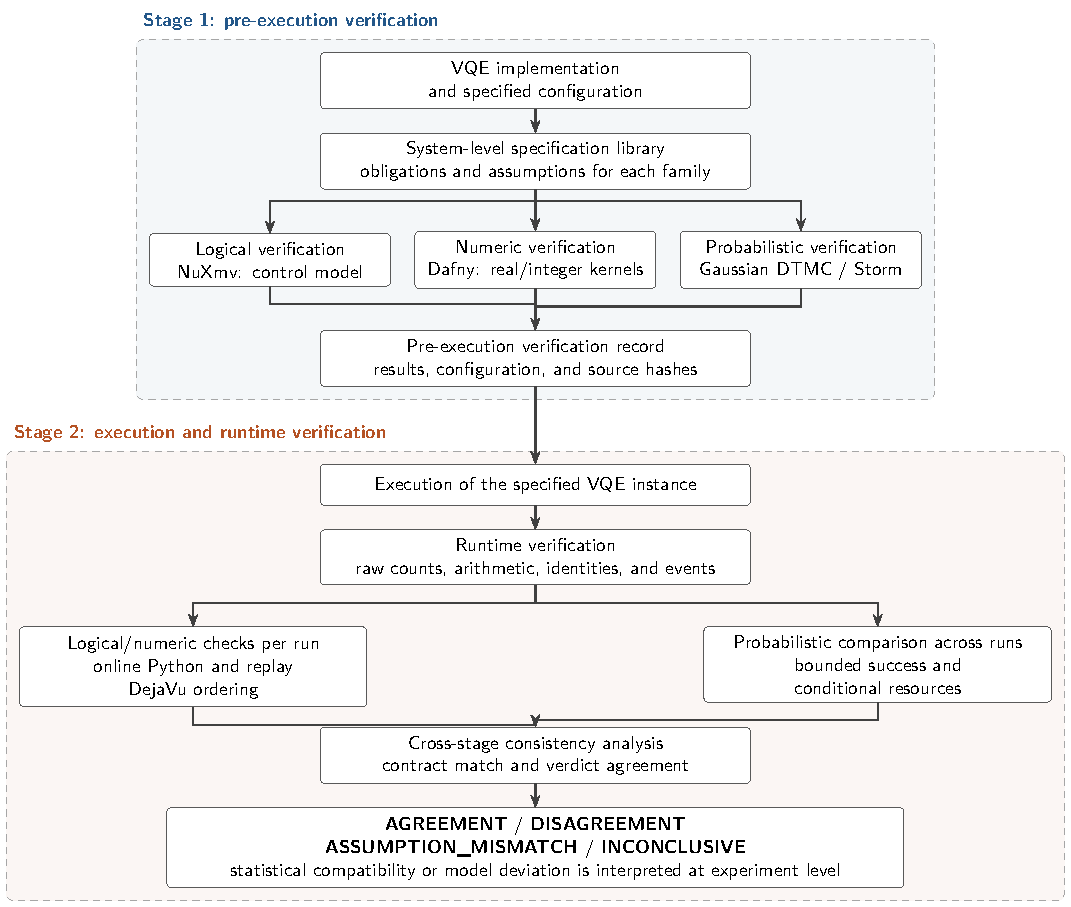
\includegraphics[width=.94\textwidth]{figures/architecture.pdf}
\caption{Four verification layers organized into two stages for the specified VQE instance. Logical, numeric, and probabilistic verification produce results before execution using their own formalisms. Runtime verification checks logical and numeric obligations for individual runs and compares probabilistic predictions with repeated executions. The verification record associates these checks with the same configuration and source files. The displayed verdict names match the implementation. Probabilistic verdicts are interpreted under the stated assumptions and statistical decision rule.}
\label{fig:architecture}
\end{figure*}

Table~\ref{tab:mapping} maps the specifications to prospective checks and runtime observations. For a numeric contract, the checker interprets concrete counts and optimizer inputs as the kernel's mathematical inputs, checks the preconditions, and compares the observed output with the specified arithmetic. The Dafny proof establishes the kernel's mathematical property. Runtime reconstruction assesses that property on observed Python inputs and outputs. For a probabilistic requirement, the runtime counterpart is an estimate over repeated executions of the specified process.

\begin{table*}[!t]
\centering\footnotesize
\caption{System-level specification mapping. Each row identifies an obligation, its prospective verification, the corresponding runtime observations, and the interpretation of their relationship. The assumption--obligation scope determines the contract match.}
\label{tab:mapping}
\begin{tabularx}{\textwidth}{@{}p{.04\textwidth}>{\raggedright\arraybackslash}p{.20\textwidth}>{\raggedright\arraybackslash}p{.25\textwidth}>{\raggedright\arraybackslash}p{.25\textwidth}Y@{}}
\toprule
ID & Obligation & Pre-execution verification & Runtime observations & Cross-stage interpretation \\
\midrule
L1 & Complete measurements before energy aggregation & NuXmv: aggregation implies three group completions & Unique candidate/group records and DejaVu past-group facts & Ordering agreement when required records are present \\
L2 & Candidate validation before optimizer commitment & NuXmv: selection/commit requires three ready candidates & Three validation events precede commit, with consumed scores recorded & Ordering agreement with fail-stop enforcement \\
L3 & Current evaluation and parameter provenance & NuXmv: epoch equality and readiness reset & Run/iteration/evaluation identities, indices, angles, successors & Runtime checks strengthen the epoch abstraction \\
L4 & Terminal closure and declared stopping reason & NuXmv: absorbing terminals and budget bounds & No later activity, with reason checked against oracle/budget & Agreement for shared properties. Reason is checked at runtime \\
N1 & Expectations consistent with raw counts & Dafny normalization kernel and range bound & Exact parity reconstruction and count totals & Agreement under trusted basis and parity mapping \\
N2 & Energy uses declared coefficients and measurements & Dafny contribution, weighted-sum, and interval kernels & Rational reference versus contributions, total energy, actual optimizer input & Arithmetic agreement within the specified tolerance \\
N3 & Physical shots counted consistently & Dafny natural-number list accumulation & Unique group executions, allocations, cumulative totals & Agreement under group-identity assumptions. Changed shots invalidate the stochastic setup \\
N4 & Valid candidates and deterministic selection & Dafny modular wrap and integer argmin/tie priority & Recomputed candidate indices, scores, chosen successor & Agreement under trusted angle/gate interpretation \\
P1 & Bounded success probability & Storm reachability of the Gaussian DTMC & First-success frequencies and Wilson intervals & Statistical compatibility under the model's assumptions \\
P2 & Iterations conditional on bounded success & Python propagation of the same Gaussian kernel & Mean first-success iteration and bootstrap interval & Supporting comparison with multiplicity adjustment \\
P3 & Shots conditional on bounded success & Fixed shot allocation times P2 & Successful-path shots at fixed shots/iteration & Derived from P2 \\
\bottomrule
\end{tabularx}
\end{table*}

\subsection{VQE Instance and Configuration}
\label{sec:instance}
The experiment uses a two-qubit benchmark operator published in IBM's VQE example~\cite{ibmvqe}, written in $q_1\otimes q_0$ order:
\begin{equation}
 H=0.398\,YZ-0.398\,ZI-0.0113\,ZZ+0.181\,XX.
 \label{eq:hamiltonian}
\end{equation}
The project's supplied \texttt{vqe\_qiskit.py} directly constructs these Pauli terms and coefficients, which match the published example. The implementation uses that operator as input rather than deriving it from electronic integrals. Neither the project nor the cited two-qubit example supplies a molecular geometry, orbital basis, or fermion mapping for this operator. We therefore call it the \emph{IBM two-qubit VQE benchmark}. Internal ``h2'' filenames are legacy identifiers. Its reference minimum eigenvalue is $E_{\rm ref}=\GroundEnergy$ in the operator's numerical units, and the success target is defined relative to this value.

The circuit follows the example's four-parameter \texttt{efficient\_su2} construction~\cite{ibmvqe}. It applies H to both qubits, the first pair of RZ rotations, Y to both, CX$(0\!\to\!1)$, H to both, the second pair of RZ rotations, and Y to both. Four integer indices $z$ give angles $\theta_j=2\pi z_j/\GridSize$, with wrap-around.

We use cyclic coordinate search to make the finite-shot selection rule explicit and representable in a finite-state probabilistic model. This derivative-free method chooses among measured objective values, consistent with the general direct-search approach~\cite{kolda2003}. At each iteration it remeasures the current, minus-one, and plus-one candidates on the selected coordinate, then chooses the smallest integer energy score. Ties prefer current, then minus, then plus. The coordinate cycle and fixed grid make candidate validity, tie handling, measurement accounting, and stochastic transitions directly checkable. The choice serves this verification experiment. Performance comparisons with other VQE optimizers are outside the evaluation. The integer coefficients are the declared decimal coefficients scaled by $10^4$.

\begin{table}[!t]
\centering\footnotesize
\caption{VQE configuration used for the two-stage evaluation. One iteration contains three candidate energy evaluations and nine measurement-group executions.}
\label{tab:configuration}
\begin{tabularx}{\columnwidth}{@{}p{.43\columnwidth}Y@{}}
\toprule
Item & Declared value \\
\midrule
Parameter grid & $z\in\{0,\ldots,\GridSize-1\}^4$, with \GridPoints points \\
Initial index & $(3,11,6,14)$ \\
Coordinate cycle & $(0,1,2,3)$ \\
Measurement groups & $\{ZI,ZZ\}$, $\{YZ\}$, $\{XX\}$ \\
Shots/group/candidate & \ShotsPerGroup \\
Physical shots/iteration & \ShotsPerUpdate \\
Iteration bound & $K=\UpdateBound$ \\
Maximum shots/run & \MaxShotsRun \\
Success & $E_{\rm ideal}(z)-E_{\rm ref}\leq\GapThreshold$ \\
Baseline executions & \BaselineRuns with separate seeded streams \\
Environment & Ideal Born probabilities and finite-shot multinomial counts \\
Numeric tolerance & $10^{-12}$ for energy and expectations \\
Gaussian integration & \QuadraturePoints-node Gauss--Hermite quadrature \\
Intervals & 95\% Wilson and \BootstrapSamples bootstrap resamples \\
\bottomrule
\end{tabularx}
\end{table}

Table~\ref{tab:configuration} specifies the execution boundary. An \emph{iteration} completes one three-candidate selection, while an \emph{evaluation} estimates the energy of one candidate. A run stops when the selected point first satisfies the ideal-energy success predicate or when it exhausts the iteration budget. An online contract violation triggers error closure. The success oracle uses exact simulation of the selected point and is available within this simulator experiment. Hardware-observed convergence requires a stopping policy based on measurable quantities. There are \SuccessPoints successful grid points. Every unsuccessful run remains in the probability denominator and consumes its budget.

\section{Layered Verification Methodology}
\label{sec:methods}
\subsection{Logical Verification}
NuXmv~\cite{nuxmv} checks a finite controller with measurement-group counters, candidate readiness, an iteration counter, and epoch flags. Nondeterministic inputs represent measurement completion, success, and environment errors. The model abstracts numeric energies and quantum states so that it can examine ordering and control flow. Representative LTL properties are
\begin{align}
 &\mathbf G(\mathrm{aggregate}\Rightarrow\mathrm{groups}=3),\nonumber\\
 &\mathbf G(\mathrm{select}\lor\mathrm{commit}\Rightarrow\mathrm{ready}=3),\nonumber\\
 &\mathbf G(\mathrm{commit}\Rightarrow\mathrm{energyEpoch}=\mathrm{epoch}).
 \label{eq:logical}
\end{align}
Readiness resets at the next iteration, and terminal states are absorbing. The procedure generates the controller using the specified iteration bound, runs NuXmv, and stores each property and verdict. The result is exhaustive for the encoded model.

L4 covers terminal absorption, the counter value at budget termination, and commitment below the bound. The audit found that redirecting either the success or budget branch to abort leaves the checked properties true. The prospective result therefore establishes those three conditions. Correct selection of the termination reason is an additional obligation checked at runtime. This distinction identifies the exact part of the specification supported by each stage.

\subsection{Numeric Verification and Its Runtime Match}
\label{sec:numeric}
Dafny~\cite{dafny} proves kernels with mathematical real and integer semantics. A normalization routine assumes a positive shot count and an admissible event count. Weighted-sum routines assume matching term sequences and expectations in $[-1,1]$, and establish
\begin{equation}
 -\sum_i|c_i|\leq\sum_i c_i\hat e_i\leq\sum_i|c_i|.
 \label{eq:numericbound}
\end{equation}
Additional kernels accumulate natural-number shot records, preserve the grid under modular wrap, and choose the minimum integer score with the declared tie priority. The verification record associates the proof logs with the source modules.

Runtime matching reconstructs expectations from raw measurements. For outcome counts $n_{g,o}$ in group $g$, let $s_{i,o}\in\{-1,+1\}$ be the declared Pauli parity. The reference values are
\begin{equation}
 \hat e_i^{\rm ref}=\frac{\sum_o s_{i,o}n_{g,o}}{\sum_o n_{g,o}},
 \qquad E^{\rm ref}=\sum_i c_i\hat e_i^{\rm ref}.
 \label{eq:runtime-reference}
\end{equation}
The checker reconstructs these as exact rational numbers and compares the concrete floating-point expectations, contributions, and energy within the specified tolerance. It also checks the integer scores and the actual values consumed by the optimizer. The contract match connects the kernel's mathematical obligation to the observed inputs and outputs. The Dafny proof applies to the mathematical kernel, and the runtime check assesses floating-point conformance for each observed evaluation.

The normalization lemma uses a single-event count form and assumes the supplied parity interpretation. The shot-accumulation proof establishes a list sum under the assumption that entries identify distinct physical executions. Runtime identity and completeness checks assess these input conditions under faithful instrumentation. Missing inputs prevent reconstruction. Changed shot allocations invalidate the specified probabilistic configuration. The runtime checker must therefore assess both the input assumptions and the arithmetic consequence.

\subsection{Probabilistic Verification}
\label{sec:probabilistic}
For each candidate, the Gaussian abstraction matches the ideal mean energy and the shot-estimator variance. Terms measured in the same group retain their covariance:
\begin{equation}
 \sigma^2(z)=\frac{1}{N_g}\sum_g
 \operatorname{Var}_{\rm Born}\!\left(\sum_{i\in g}c_i s_i\right),
 \label{eq:variance}
\end{equation}
where all groups receive $N_g=\ShotsPerGroup$ shots. The experiment samples groups, candidate measurements, and repeated executions independently. Terms measured within a group share outcomes, so their covariance contributes to the variance, as in grouped VQE energy estimation~\cite{mcclean2016,tilly2022}. Approximating a candidate energy by $X_j\sim\mathcal N(\mu_j,\sigma_j^2)$ gives its selection probability
\begin{equation}
 \Pr(j=\operatorname*{argmin}_\ell X_\ell)
 =\int f_j(x)\prod_{\ell\ne j}[1-F_\ell(x)]\,dx.
 \label{eq:selection}
\end{equation}
The implementation evaluates this integral using the configured quadrature and normal-CDF approximation, then normalizes the transition probabilities. The continuous model assigns zero probability to ties. Discrete finite-shot execution uses the specified tie rule.

The DTMC state is the parameter-grid point and next coordinate phase. Success states are absorbing. Storm~\cite{storm} checks
\begin{equation}
 p_G(k)=\Pr_G(T\leq k)
 \quad\text{using }\mathrm{P}_{=?}[\mathrm F^{\leq k}\ \mathrm{success}].
 \label{eq:reachability}
\end{equation}
Storm exhaustively checks the constructed Gaussian DTMC. Empirical executions assess how well its prediction describes the finite-shot process. Python forward propagation of the same kernel produces the full cumulative curve and first-success distribution. P2 is $\mathbb E_G[T\mid T\leq K]$, and P3 multiplies P2 by the fixed shots per iteration. These quantities are computed by Python propagation conditional on bounded success. Total expenditure includes unsuccessful paths and is reported separately. Numerical agreement between Storm and propagation assesses the model computation. Accuracy relative to the finite-shot process requires empirical comparison or a separate approximation-error analysis.

\subsection{Runtime Verification}
\label{sec:runtime}
The executor records preparation and iteration context, raw group counts, candidate evaluations, successful numeric checks, optimizer commits, and terminal closure. Python checks each emitted event synchronously and stops the run when a problem appears. It checks current identities, complete measurements, arithmetic, consumed scores, successor parameters, resource totals, and terminal reasons. The implementation records a commit and assigns the successor before checking acceptance. Thus a failed check stops subsequent activity after the event has been emitted.

Saved traces are replayed with the same Python checker class to reproduce the online verdicts. A separately compiled DejaVu monitor~\cite{dejavu} replays five temporal properties: complete groups before aggregation, validation before commit, energy after iteration start, validation after energy, and closure after stopping. This provides an independent implementation of the ordering checks. Arithmetic verification and count-source authenticity remain outside those temporal properties. The runtime cost evaluation in Section~\ref{sec:runtime-cost} uses a synchronous ask/tell protocol, in which the optimizer submits candidates and receives acknowledgment of validated results.

\section{Individual Layer Evaluation}
\label{sec:individual}
\subsection{Experimental Setup}
All evaluations use the IBM two-qubit benchmark in Eq.~\eqref{eq:hamiltonian}, except the larger Heisenberg trace used to exercise numeric checking. Each layer evaluates the object relevant to its specifications. The logical study varies the controller's iteration bound and observable count. The numeric study verifies arithmetic kernels and checks stored term-level records. The probabilistic study measures the size and checking cost of Gaussian DTMCs over the finite grid. The runtime study measures monitoring cost and checks sampled simulator and hardware executions.

For logical verification, NuXmv evaluates the refined controller and its phase-reachability queries. Its budget terminal uses an abort label. Numeric checking uses version 2.0 of the trace checker on a two-qubit Estimator trace and an exact-estimate Heisenberg trace. Both record expectations and contributions, without raw measurement counts. These traces support checking the reported arithmetic and record structure.

The probabilistic scalability study fixes the circuit, grid, initial point, measurement groups, and shot allocation in Table~\ref{tab:configuration}. It varies the horizon of a reachable, time-unrolled Gaussian DTMC. Success uses the specified ideal-energy gap. Model sizes are deterministic counts, construction has one timing measurement per horizon, and checking uses the median of three tool timings.

Runtime timing uses Qiskit's StatevectorSampler, four independent Pauli submissions per evaluation, and \ShotsPerGroup shots per term. An ask/tell pattern-search optimizer uses an initial step of $0.4$, a shrink factor of $0.5$, and the recorded energy-stability rule: tolerance $0.005$ for three successive checks after at least ten evaluations. The cost sweep fixes the workload seed at seven and evaluates counts from ten to fifty in increments of ten. It has \TimingWarmupsPerCell warm-ups and \TimingRepetitions measured repetitions per condition/count. Independent-condition bootstrap resampling gives uncertainty intervals for the medians and added time. The hardware assessment uses the recorded \texttt{ibm\_marrakesh} execution and its simulator counterpart. Their results concern monitored conformance and declared termination.

Section~\ref{sec:crosslayer} specifies the two-stage evaluation using the fixed configuration in Table~\ref{tab:configuration} and repeated finite-shot executions. All reported numerical text, tables, and plots are generated from the corresponding source artifacts.

\subsection{Logical and Numeric Outcomes}
The refined controller has \LegacyLogicalProperties true properties in its NuXmv output and \PhaseQueries positive phase-reachability queries. For the iteration-bound/term-count pairs \LogicalScalingPairs, wall-clock measurements are respectively \LogicalScalingTimes~s. Every configuration returns the same \LegacyLogicalProperties true properties and zero false properties. These are single local timing measurements of bounded controllers, so the observed costs apply to the tested configurations.

For the controller used in the two-stage evaluation, \LogicalProperties logical properties hold. Three Dafny invocations report \DafnyChecks verified units with zero errors. A verified unit is a tool-reported proof task. The specification mapping identifies how these tasks support N1--N4, and the result manifest records their distribution across modules.

The numeric checker accepts all \EstimatorRecords records of the \EstimatorQubits-qubit, \EstimatorTerms-term Estimator trace and all \HeisenbergRecords records of the \HeisenbergQubits-qubit, \HeisenbergTerms-term exact-estimate Heisenberg trace. These results demonstrate arithmetic and record conformance for the supplied values, including a larger term list. Raw-count reconstruction requires measurement records beyond the fields available in either trace. Timing scaling and optimization success are outside this trace assessment. Synthetic fixtures remain classified as checker inputs.

\subsection{Probabilistic Model Size and Cost}
\label{sec:modelcost}
The scalability study builds a reachable, time-unrolled DTMC for each iteration bound. It merges successful paths into an absorbing success state and exhausted paths into an absorbing timeout state. Figure~\ref{fig:storm-scalability} shows the model sizes and costs. At the largest bound, it contains \ScaleMaxStates states and \ScaleMaxTransitions transitions. The homogeneous grid/coordinate-phase DTMC used for the two-stage evaluation has \ModelStates states and \ModelTransitions transitions. Its fixed representation supports queries at different horizons, while time unrolling explicitly includes the iteration depth in the state space.

\begin{figure}[!t]
\centering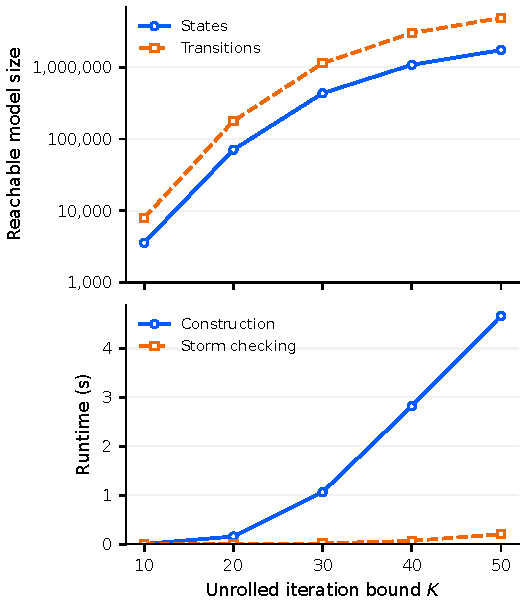
\includegraphics[width=\columnwidth]{figures/storm-scalability.pdf}
\caption{Time-unrolled Gaussian DTMC scalability at the grid and shot allocation in Table~\ref{tab:configuration}. Top: reachable states and transitions, with a logarithmic vertical axis. Bottom: construction time from one measurement and median Storm checking time from three recorded invocations at each bound. Construction excludes Gaussian-kernel preparation, and checking excludes parsing. A displayed zero is below the tool's timing resolution. This representation includes iteration depth, whereas the homogeneous phase DTMC used in Section~\ref{sec:crosslayer} has fixed size.}
\label{fig:storm-scalability}
\end{figure}

The cost panel separates construction from model checking. Source artifacts contain per-depth state counts, timings, the CSV summary, metadata, and generation source. The exported explicit scalability models are unavailable. The reported growth and costs can therefore be reconstructed from the recorded metadata and measurements, with direct model-file inspection available for the homogeneous DTMC.

The FakeJakarta density-matrix study records \NoisySuccess/\NoisyRuns successes (\NoisyPercent\%). It assesses robustness under backend noise and compiled circuits. Those conditions extend beyond the ideal-Born assumptions of the Gaussian model, so the result describes noisy execution under its own configuration. The probability comparison in Section~\ref{sec:crosslayer} uses ideal finite-shot runs and the model's success predicate.

\subsection{Runtime Cost and Hardware Results}
\label{sec:runtime-cost}
The runtime cost study has \TimingWarmup warm-ups and \TimingMeasured measured runs under the setup described above. Reusing the workload seed holds the sampled trajectory fixed while repetitions measure timing variation.

Figure~\ref{fig:runtime-overhead} reports total runtime and the difference of condition medians. Verified timing includes VQE setup and sampling, monitor startup, synchronous checking and acknowledgments, trace and measurement-record persistence, and finalization. Baseline post-run serialization, fidelity analysis, and offline replay are excluded from the timing boundary. Bootstrap samples independently resample each condition's measured times. The intervals describe uncertainty in the timing summaries for this fixed workload.

\begin{figure}[!t]
\centering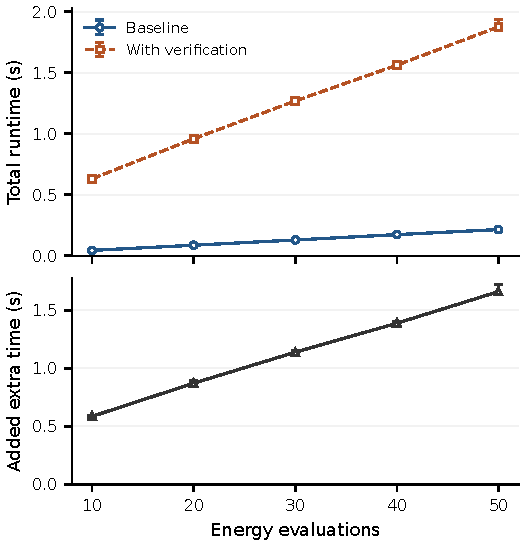
\includegraphics[width=\columnwidth]{figures/runtime-overhead.pdf}
\caption{Simulator runtime cost with synchronous ask/tell monitoring. Top: baseline and verified medians. Bottom: verified median minus baseline median. Error bars are 95\% percentile bootstrap intervals from 10,000 independent-condition resamples, using \TimingRepetitions measured runs per condition/count after \TimingWarmupsPerCell warm-ups. Timing covers setup, execution, online checking and persistence, and finalization. Baseline post-run serialization, fidelity analysis, and offline replay are excluded. Repetitions use the same workload seed.}
\label{fig:runtime-overhead}
\end{figure}

At the largest tested count, the baseline median is \TimingBaselineFinal~s, the verified median is \TimingVerifiedFinal~s, and the added median time is \TimingAddedFinal~s (\TimingRelativeFinal\% relative increase). These measurements show substantial relative overhead on this fast simulator workload. Estimating overhead for the cyclic-grid executor would require repeated uninstrumented timings alongside its monitored executions. A systematic numeric-verification cost study is also unavailable.

Table~\ref{tab:hardware} reports the sampled simulator and \texttt{ibm\_marrakesh} executions and their online/replay outcomes. Both terminate at the evaluation budget. Acceptance supports observed event ordering, arithmetic, resource accounting, and record completeness. These properties concern the ask/tell workflow under its simulator or hardware conditions. The Gaussian search prediction is assessed under the cyclic-grid configuration in Section~\ref{sec:crosslayer}.

\begin{table}[!t]
\centering\footnotesize
\caption{Runtime simulator and hardware results verified against stored hashes and reports. ``pass/pass'' denotes online/replay conformance. Both executions terminate at the evaluation budget.}
\label{tab:hardware}
\begin{tabular}{@{}lrrrl@{}}\toprule
Execution & Evals. & PUBs & Shots & Online/replay \\
\midrule
statevector\_sampler & 50 & 200 & 204,800 & pass/pass \\
ibm\_marrakesh & 50 & 200 & 204,800 & pass/pass \\
\bottomrule


\end{tabular}
\end{table}

\section{Cross-Layer Relationships and Agreement}
\label{sec:crosslayer}
\subsection{Goals and Procedure}
The two-stage evaluation examines whether the properties established before execution correspond to the obligations checked during execution, and whether their results agree within the stated assumptions. It fixes the circuit, operator, parameter grid, candidate rule, measurement groups, shot allocation, success predicate, and iteration bound in Table~\ref{tab:configuration}. It also examines how controlled faults change the verification outcomes. The evaluated claim is consistency of the specified workflow across the two stages.

Stage 1 generates and checks the controller with NuXmv, verifies the numeric modules with Dafny, constructs the Gaussian kernel and DTMC, and runs Storm at the specified checkpoints. It also compiles the temporal monitor and records the results, configuration, and source hashes. Stage 2 checks that the execution uses this record, then performs \BaselineRuns ideal-Born finite-shot runs with independently seeded count streams. It stores raw counts and all values consumed by the optimizer, checks events online, and replays the traces. Each run stops at first success or at $K=\UpdateBound$ iterations. The ideal-energy gap defines success, as in the Gaussian model. Error closure handles online violations. No backend noise is introduced in this comparison.

For logical and numeric obligations, the comparison relates each prospective property result to the check on every observed run. The implementation labels satisfaction \texttt{AGREEMENT}, violations \texttt{DISAGREEMENT}, invalid assumptions \texttt{ASSUMPTION\_MISMATCH}, and unavailable checks \texttt{INCONCLUSIVE}. The meaning of each result follows its specification mapping. Numerical tolerances govern deterministic conformance. Stage 2 is gated on successful prospective verification, which restricts the evaluated combinations to executions authorized by Stage 1.

Probabilistic comparison operates on repeated executions. P1 compares the Gaussian reachability probability with the fraction reaching success by each checkpoint, including unsuccessful runs in the denominator. The probability at $K$ is the primary comparison. Pointwise 95\% Wilson intervals quantify binomial uncertainty~\cite{wilson}. P2 compares iterations conditional on bounded success using the original \BootstrapSamples-resample percentile-bootstrap interval. P3 applies the fixed shots per iteration to that quantity. A stochastic run that exhausts its budget is one permitted outcome of this bounded-success specification.

The supporting analysis computes two-sided score-test $p$-values at the nonzero-probability checkpoints and a normal-approximation test for P2. Holm adjustment~\cite{holm} controls multiplicity for that family at $\alpha=0.05$. The early zero-probability checkpoints are structurally uninformative, and P3 is derived from P2. This post-audit interpretation uses the existing observations and intervals. The comparison tests compatibility at the available sample size, without a preregistered equivalence margin.

\subsection{Logical and Numeric Verification Agreement}
Table~\ref{tab:contract-results} gives the prospectively established property and runtime count for each logical and numeric obligation. All observed baseline obligations agree on \BaselineRuns runs under the mapping's assumptions. The result establishes conformance of these observed executions. L4 agreement covers terminal absorption and bound conditions at both stages. The stronger termination-reason obligation is assessed at runtime.

\begin{table*}[!t]
\centering\footnotesize
\caption{Logical and numeric results by obligation. The listed prospective properties have successful tool outputs, and the runtime column counts agreeing baseline runs. Agreement is interpreted under Table~\ref{tab:mapping}'s assumptions. L4's prospective scope covers terminal absorption and budget bounds. Correct termination reasons are checked at runtime.}
\label{tab:contract-results}
\begin{tabularx}{\textwidth}{@{}p{.045\textwidth}p{.44\textwidth}p{.14\textwidth}Y@{}}\toprule
ID & Prospectively established scope & Runtime agreement & Cross-stage classification \\
\midrule
L1 & Group-completeness counter & 400/400 & Agreement under mapping \\
L2 & Validation-readiness counter & 400/400 & Agreement under mapping \\
L3 & Epoch and readiness reset & 400/400 & Agreement under mapping \\
L4 & Terminal absorption and budget bounds & 400/400 & Qualified agreement \\
N1 & Normalization kernel with parity assumed & 400/400 & Agreement under mapping \\
N2 & Real weighted sum and bound & 400/400 & Agreement under mapping \\
N3 & List sum with group identity assumed & 400/400 & Agreement under mapping \\
N4 & Wrap and integer tie-priority selection & 400/400 & Agreement under mapping \\
\bottomrule


\end{tabularx}
\end{table*}

Raw-count reconstruction covers \TotalEvaluations candidate evaluations and \TotalMeasurements group executions. The maximum observed energy reconstruction error is $\EnergyError$, below the specified tolerance. Expectation reconstruction has zero observed error. Total physical consumption is \TotalShots shots across \TotalUpdates optimizer iterations. Python online and replay verdicts agree for every run, and all baseline runs pass the DejaVu temporal replay. These counts quantify the checked observations under the logical and numeric specifications.

\subsection{Gaussian Prediction and Finite-Shot Execution}
\label{sec:probability-results}
Figure~\ref{fig:probability-comparison} compares the Gaussian first-success curve with empirical execution using the same success predicate. Forward propagation of the Gaussian kernel produces the curve, and Storm independently checks the specified checkpoint probabilities. Their maximum recorded numerical difference is $\StormDifference$. The maximum quadrature row-normalization correction is $\QuadratureCorrection$. These quantities assess numerical processing of the constructed model. The empirical comparison assesses its prediction for finite-shot execution.

\begin{figure}[!t]
\centering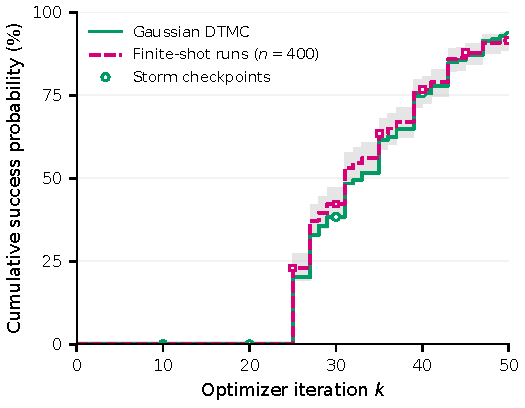
\includegraphics[width=\columnwidth]{figures/probability-comparison.pdf}
\caption{Cumulative probability of first satisfying $E_{\rm ideal}(z)-E_{\rm ref}\leq\GapThreshold$ versus optimizer iteration. The solid staircase is Gaussian-DTMC forward propagation, circles are Storm checkpoints, and the dashed staircase summarizes \BaselineRuns independently seeded ideal-Born finite-shot runs with \ShotsPerGroup shots per group/candidate. The shaded region gives pointwise 95\% Wilson intervals at each iteration. It is not a simultaneous confidence band. Both processes use the same success predicate, candidate rule, and resource configuration.}
\label{fig:probability-comparison}
\end{figure}

At the primary bound, \SuccessRuns/\BaselineRuns runs succeed and \BudgetRuns terminate normally at budget. The empirical probability is \PrimaryEmpiricalPercent\%, with Wilson interval [\PrimaryCILower\%, \PrimaryCIUpper\%], compared with \PrimaryModelPercent\% modeled probability. The absolute difference is \PrimaryDeviationPP percentage points. Table~\ref{tab:probabilities} gives exact checkpoint counts, intervals, deviations, and supporting comparisons with multiplicity adjustment. Agreement here denotes statistical compatibility at the tested resolution.

\begin{table*}[!t]
\centering\footnotesize
\caption{P1 results for the specified two-stage evaluation. Probabilities and Wilson limits are percentages, and deviations are percentage points. Holm values adjust the informative checkpoint and P2 comparisons jointly. The early zero-probability checkpoints are structural.}
\label{tab:probabilities}
\begin{tabular}{@{}rrrrlrr@{}}\toprule
$k$ & Successes/runs & Model (\%) & Empirical (\%) & Wilson 95\% (\%) & $|\Delta p|$ (pp) & Holm $p$ \\
\midrule
10 & 0/400 & 0.00 & 0.00 & [0.00, 0.95] & 0.00 & -- \\
20 & 0/400 & 0.00 & 0.00 & [0.00, 0.95] & 0.00 & -- \\
30 & 169/400 & 38.39 & 42.25 & [37.51, 47.14] & 3.86 & 0.338 \\
40 & 307/400 & 75.63 & 76.75 & [72.37, 80.62] & 1.12 & 0.627 \\
50 & 366/400 & 92.80 & 91.50 & [88.36, 93.85] & 1.30 & 0.627 \\
\bottomrule


\end{tabular}
\end{table*}

P2 is \PModelMean modeled iterations conditional on success versus \PEmpiricalMean empirical iterations, with the original percentile-bootstrap interval [\PMeanLow, \PMeanHigh]. Table~\ref{tab:conditional} preserves that interval, which does not contain the model mean. Marginal interval containment was the automated report's decision rule. The post-audit analysis interprets the supporting comparisons jointly: the raw P2 $p$-value is \PMeanRawP, becoming \PMeanAdjustedP after Holm adjustment. All informative comparisons are compatible at the family level. Thus P2 and its derived P3 result agree under the stated statistical comparison. The source report's original labels remain preserved for provenance. Statistical compatibility has the scope of this test and sample size, rather than a claim of distributional equivalence.

\begin{table*}[!t]
\centering\footnotesize
\caption{Resources conditional on bounded success in the two-stage evaluation, based on \SuccessRuns successful executions. Intervals are the original 95\% percentile-bootstrap intervals from \BootstrapSamples resamples. P2 is statistically compatible after Holm adjustment. P3 scales P2 by \ShotsPerUpdate shots/iteration and is therefore a derived result.}
\label{tab:conditional}
\begin{tabular}{@{}lrrlrl@{}}\toprule
Quantity / unit & Model mean & Empirical mean & Bootstrap 95\% & Absolute deviation & Holm $p$ \\
\midrule
P2: iterations & 33.111 & 32.290 & [31.579, 32.995] & 0.822 & 0.094 \\
P3: shots & 305,152.7 & 297,581.1 & [291,034.2, 304,077.6] & 7,571.6 & derived \\
\bottomrule


\end{tabular}
\end{table*}

Including unsuccessful runs, mean expenditure is \UnconditionalEmpirical iterations versus \UnconditionalModel modeled iterations. Total shot consumption includes budget-terminated paths, whereas P2 and P3 describe successful paths. The primary probability comparison's approximate normal-theory deviation detectable at 80\% power is \DetectablePP percentage points at this sample size. This local planning approximation describes statistical resolution. An equivalence claim would require a declared margin and corresponding test. Supporting checkpoints are correlated, and the confidence band is pointwise.

\subsection{Faults and Cross-Stage Discrepancies}
\label{sec:faults}
Figure~\ref{fig:fault-discrepancies} reports the full logical and numeric verdict vector. The matrix shows which obligations respond to each fault, with distinct symbols for violations, changed assumptions, and unavailable checks. There are \FaultClasses fault scenarios, each repeated \FaultRepetitions times, for \FaultRuns tests. Execution faults use the first iteration/candidate boundary. The missing-count scenario deletes counts from a saved trace while preserving the corresponding control execution. It assesses how the checker handles incomplete records.

\begin{figure*}[!t]
\centering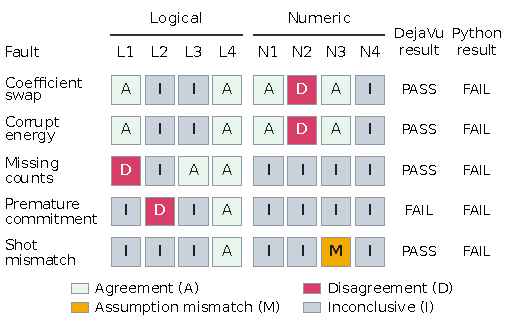
\includegraphics[width=\textwidth]{figures/fault-discrepancies.pdf}
\caption{Fault verdict matrix for \FaultClasses scenarios, each repeated \FaultRepetitions times with different count streams. Every repetition within a row has the displayed vector. Colors and letters indicate A: AGREEMENT, D: DISAGREEMENT, M: ASSUMPTION\_MISMATCH, and I: INCONCLUSIVE. ``Expected verdict'' counts the specified target-obligation result, including an inconclusive result for missing counts. ``DejaVu pass'' counts acceptance by the independent temporal replay. Missing counts are removed from a saved trace. Its L1 D reflects the checker's treatment of incomplete records and does not establish a physical ordering violation.}
\label{fig:fault-discrepancies}
\end{figure*}

Premature commitment is caught by Python and DejaVu ordering checks. Altering the energy or coefficient pairing violates N2 while temporal properties pass, illustrating their complementary scopes. A shot-allocation change produces an N3 assumption mismatch and makes the probabilistic comparison inapplicable. The injector configures this applicability label, so it records which stochastic assumptions the fault changes.

Missing counts make numeric reconstruction inconclusive. The checker also records an L1 disagreement because its completeness condition treats unavailable records as missing measurements. A deleted record alone does not establish that the original execution aggregated too early. The full vector exposes this classification limitation alongside the expected target detections. The suite covers the specified fault classes at one injection boundary. Terminal-boundary faults, stale inputs, and additional injection sites require further tests.

\subsection{Summary of Verification Results}
The evaluation begins with properties of the controller, arithmetic kernels, and Gaussian process, then checks the corresponding obligations on executions of the specified configuration. The mapping makes the role of each verification layer explicit. Logical results describe allowed ordering, numeric results describe calculations under input assumptions, and probabilistic results describe bounded search. Runtime checking determines whether the logical and numeric obligations hold in each run, while repeated executions assess the probabilistic predictions.

The baseline agreement supports this connection at the level of the established properties. Logical and numeric checks accept every observed baseline run, and the bounded-success and conditional-resource comparisons are statistically compatible under the stated analysis. P3 follows P2 because shots per iteration are fixed. Successful comparisons therefore depend on the meaning and scope of the requirement, as well as on the reported verdict. L4 illustrates the distinction: both stages assess terminal closure and budget bounds, while correct termination reasons have runtime support.

Fault results show why the four aspects are useful together. Temporal checking detects premature commitment, whereas numeric reconstruction detects energy and coefficient errors that preserve temporal order. Changed shot allocations identify assumptions that must be restored before comparing stochastic outcomes. Missing counts reveal a further requirement for the implementation: it must distinguish incomplete observations from observed violations. Preserving the full verdict vector exposes this limitation.

The combined assessment thus provides traceable agreement among heterogeneous verification results within the tested configuration. Its practical value is the ability to locate the affected obligation and the limits of its support. Model growth and runtime costs in Section~\ref{sec:individual} establish the measured expense of the corresponding verification components. Extending the conclusions requires stronger termination properties, broader fault coverage, and evaluations under larger or noisy execution models.

\section{Related Work}
VQE and variational hybrid algorithms combine classical decisions with quantum measurements~\cite{peruzzo2014,mcclean2016}. Reviews of VQE examine measurement strategies, optimization, noise, and their impact on practical performance~\cite{tilly2022}. Direct-search literature provides the optimization context for choosing candidates using objective values~\cite{kolda2003}. Here, the finite-grid search makes these decisions explicit enough to model their probability and inspect their execution.

NuXmv, Dafny, Storm, and DejaVu provide established methods for model checking, deductive verification, probabilistic analysis, and temporal monitoring~\cite{nuxmv,dafny,storm,dejavu}. We use these methods according to the requirements of each layer. The contribution is a specification mapping and two-stage procedure that relates their results to an implemented VQE workflow and identifies the scope of agreement.

Statistical methods quantify the uncertainty in empirical comparison. Wilson intervals describe a binomial proportion~\cite{wilson}, and Holm adjustment controls the family-wise rejection rate for a specified family of tests~\cite{holm}. Their role is to assess compatibility between model predictions and sampled outcomes. The conditional-resource comparison illustrates why a marginal interval and a family-level interpretation answer different statistical questions.

\section{Discussion and Limitations}
\label{sec:limitations}
\emph{Verification scope.} NuXmv is exhaustive for its encoded controller. Dafny proves kernels under mathematical semantics and preconditions. Storm is exhaustive for the constructed Gaussian DTMC. Runtime checking covers observed instrumented traces, and repeated executions provide statistical evidence. The framework relates these scoped results through specification mappings. Establishing a formal refinement from every model to the Python program remains future work.

\emph{Trusted base.} Circuit and measurement-basis generation, bit order and parity interpretation, event instrumentation, proof tools, and the runtime reference checker are trusted. Hashes associate source and result files with the recorded experiment. Authenticating the physical origin of counts requires additional protection, particularly against consistent fabrication or relabeling. A certified bound on stochastic approximation error would also require analysis beyond the normal-CDF approximation and quadrature used here.

\emph{Generality and observability.} The two-stage evaluation uses a small two-qubit benchmark with a fixed finite grid, ideal statistics, and an exact-energy stopping oracle. Its target, optimizer, grouped measurements, and finite budget define the evaluated boundary. The hardware execution and larger numeric trace demonstrate the corresponding runtime and arithmetic checks. Extending prospective agreement to those instances requires models and specifications for their configurations and observable stopping rules.

\emph{Statistical and audit boundaries.} The P2/P3 interpretation is a post-audit reporting correction. Original marginal intervals and observations remain visible, and the sample size constrains statistical resolution. Development executions used the same seeds and are excluded from the reported sample counts. Their trajectories were already known before the recorded prospective verification, so this is an engineering evaluation rather than a blinded confirmatory study. The independent audit identified gaps in termination properties and classification of missing records. The reported scopes reflect these findings, with the experiment sources unchanged. The auditor's additional simulations support its statistical interpretation, but their saved arrays are unavailable. Their numerical summaries are therefore excluded. The reproducibility manifest also documents the unavailable scalability model exports.

\emph{Feedback scope.} The framework detects inconsistencies and supports revising assumptions or specifications before regenerating the verification record and running the next execution. This feedback is manual. The evaluated workflow gates execution on successful prospective results, and the fault scenarios cover the specified boundary.

\section{Conclusion}
The four-layer architecture organizes VQE verification around logical, numeric, probabilistic, and runtime requirements. Its two-stage framework connects properties established prospectively with the corresponding obligations checked during concrete execution of a specified configuration. The benchmark results support logical and numeric agreement within the verified scope and statistical compatibility of Gaussian predictions with repeated finite-shot executions. Fault vectors reveal complementary detection capabilities and a limitation in classifying missing records. Model-size and timing measurements quantify the cost of the evaluated components. Together, the results demonstrate a traceable assessment of heterogeneous verification methods. Future work will strengthen termination specifications, examine additional fault locations, and extend the models and runtime checks to larger instances and hardware noise.

\section*{Artifact Availability}
The local reproducibility bundle includes this source, vector figures, editable architecture source, figure-generation scripts, generated numerical tables, \path{FIGURE_PLAN.md}, \path{FIGURE_MANIFEST.md}, and \path{PAPER_RESULT_TRACEABILITY.md}. The source manifest records hashes of the verification record, models, proof logs, raw traces, and individual-layer inputs. Original experimental artifacts and the reference manuscript are preserved. The bundle is currently a local research artifact.

\bibliographystyle{IEEEtran}
\IEEEtriggeratref{4}
\bibliography{references}
\end{document}
